\documentclass[12pt]{article}

% \usepackage[brazil]{babel}
\usepackage[brazilian]{babel}
%\usepackage[latin1]{inputenc}
\usepackage[utf8]{inputenc}
\usepackage[T1]{fontenc}

\usepackage{lscape}
\usepackage{latexsym}
\usepackage{amscd}
\usepackage{amsfonts}
\usepackage{epsf}
\usepackage{times}
\usepackage{multicol}
\usepackage{makeidx}
%\input{heading.tex}
%%%%%%%%%%%%%%%%%%%%%%%%%%%%%%%%%%%%%%%%%%%%%%%%%%%%%%%%%%%%%%%%%%%%%%
\renewcommand{\contentsname}{2.\enspace Índice}
\setcounter{tocdepth}{1}
%%%%%%%%%%%%%%%%%%%%%%%%%%%%%%%%%%%%%%%%%%%%%%%%%%%%%%%%%%%%%%%%%%%%%%
%\def\FAPESP{\textsc{fapesp}}
%%%%%%%%%%%%%%%%%%%%%%%%%%%%%%%%%%%%%%%%%%%%%%%%%%%%%%%%%%%%%%%%%%%%%%
\def\BibTeX{{\rm B\kern-.05em{\sc i\kern-.025em b}\kern-.08em
    T\kern-.1667em\lower.7ex\hbox{E}\kern-.125emX}}
%%%%%%%%%%%%%%%%%%%%%%%%%%%%%%%%%%%%%%%%%%%%%%%%%%%%%%%%%%%%%%%%%%%%%%
% sizes, lengths,...
\special{papersize=21.59cm,27.94cm}
\usepackage[top=3cm,left=2cm,right=2cm,bottom=3cm]{geometry}
\linespread{1.45}
\makeindex

%\setlength{\textwidth}{40pc}
%\setlength{\textheight}{52pc}
%\setlength{\baselineskip}{2pc}
%%\setlength{\parindent}{15mm}
%\setlength{\parskip}{1pc}
%\setlength{\topmargin}{5mm}
%\setlength{\oddsidemargin}{0mm}
%\setlength{\evensidemargin}{0mm}
%\linespread{1.3}
%\setcounter{tocdepth}{2}
 
%%%%%%%%%%%%%
% Hyphenation
%%%%%%%%%%%%%
\hyphenation{mes-mo im-ple-men-ta-ção tam-bém prá-ti-ca 
             com-pli-ca-ções di-nâ-mi-ca vir-tua-li-za-ção 
             fre-quên-cia pro-ces-sa-dor}

%%%%%%%%%%%%%
% Palavra em idioma estrangeiro
%%%%%%%%%%%%%
\newcommand{\etal}{\emph{et alli}}
\newcommand{\Software}{\emph{Software}}
\newcommand{\Hardware}{\emph{Hardware}}
\newcommand{\software}{\emph{software}}
\newcommand{\softwares}{\emph{softwares}}
\newcommand{\hardware}{\emph{hardware}}
\newcommand{\DOTNET}{.NET}
\newcommand{\VLIW}{VLIW}
\newcommand{\benchmark}{\emph{benchmark}}
\newcommand{\benchmarks}{\emph{benchmarks}}
\newcommand{\laptops}{\emph{laptops}}
\newcommand{\scripts}{\emph{scripts}}

\bibliographystyle{plain}

%--------------------------------
\begin{document}

%---------------------------------------------------------------------
% Resumo em português
%---------------------------------------------------------------------
\thispagestyle{empty}
\bigskip
\bigskip
\centerline{\LARGE\bf Documento de Extração de Requisitos}
\bigskip\bigskip
\bigskip\bigskip
\bigskip\bigskip
\bigskip\bigskip
\bigskip\bigskip
\bigskip\bigskip
\bigskip\bigskip
\bigskip\bigskip
\bigskip\bigskip
\bigskip\bigskip
\bigskip\bigskip
\centerline{\large\bf Aluno: Renato César Martins - RA: 073668}
\centerline{\large\bf Aluno: Matheus Smythe Svolenski - RA: 103520}
\centerline{\large\bf Aluno: Rafael Timbó Matos - RA: 106228}
\centerline{\large\bf Professora: Ariadne M. B. R. Carvalho}
\bigskip\bigskip
\bigskip\bigskip
\bigskip\bigskip
\bigskip\bigskip
\bigskip\bigskip
\bigskip\bigskip
\bigskip\bigskip
\bigskip\bigskip
\bigskip\bigskip
\bigskip\bigskip
\centerline{\large Instituto de Computação}
\centerline{\large Universidade Estadual de Campinas}
\centerline{\large Março de 2012}
\clearpage

\section {Introdução}
\label{sec:intro}

O presente documento visa especificar os requisitos para a informatização do portal de viagens ViajarFacil.com.br. Esta página visa facilitar à utilização de serviços de viagens, fornecendo diversas opções em um único portal. O usuário do site poderá buscar por passagens aéreas, pacotes de viagem, cruzeiros e hotéis, podendo comprá-los diretamente através do site, utilizando-se de uma conta criada no mesmo.

Apenas a reserva de hotéis não poderá ser realizada diretamente através do ViajarFacil. Sendo assim, após a busca e a seleção de sua preferência, o usuário será redirecionado ao portal parceiro adequado para realizar a reserva. 

%====================================================================
\section{Glossário}
\label{sec:glossario}

{\bf Portal} - Um site na internet que funciona como centro de conteúdo para uma série de outros sites ou subsites dentro, e também fora, do domínio ou subdomínio da empresa gestora do portal.

{\bf Requisitos Funcionais} - Funcionalidades que se espera que o sistema disponibilize, de uma forma completa e consistente.

{\bf Requisitos Não-Funcionais} - Aspectos não-funcionais do sistema, como restrições nas quais o sistema deve operar (confiabilidade, tempo de resposta, segurança, portabilidade, facilidade de uso, linguagem de implementação).

{\bf Sistema} - Um conjunto de elementos interconectados, de modo a formar um todo organizado visando atingir um determinado objetivo.

{\bf Login} - Processo através do qual se controla o acesso a um sistema informático por meio de identificação e autenticação do usuário através de credenciais.

{\bf Log} -  Registro de eventos relevantes num sistema computacional, geralmente para restaurações, auditorias, diagnóstico ou histórico.

{\bf Banco de Dados} - Coleção organizada de registros relacionados, cuja interface fornece métodos organizados para coletar, manipular e transmitir dados ou informações.

{\bf Interface} - Ponto de interação em que dois componentes que funcionem de maneira distinta trocam dados e informações através de um protocolo.

{\bf Usuário} - Agente utilizador de um serviço

\clearpage
%====================================================================
\section{Definição dos requisitos de usuário}
\label{sec:req_usuario}
\subsection{Requisitos funcionais}

{\bf RF01.} O sistema deve possuir uma interface de buscas, separada para cada tipo de consulta, para que o cliente possa consultar passagens aéreas, hotéis e cruzeiros, bem como pacotes de viagem.

Informações: data da partida, data da volta, número de adultos e de crianças, local de origem e de destino da viagem, companhia aérea (exclusivo para as passagens aéreas), faixa de preço, viagem nacional ou internacional.

Regras: caso haja resultado para a consulta, o sistema deverá disponibilizar os pacotes de viagem, passagens aéreas, hotéis ou cruzeiros, com seus preços, caso não haja, informar ao cliente que não houve resultado para a consulta.

\bigskip
{\bf RF02.} Sistema de login para o usuário, para que seja possível guardar as informações do usuário no site, bem como os locais favoritos por ele escolhidos.

Informações: necessita do nome de usuário e senha para entrar. Ao cadastrar-se será necessário entrar com mais informações: nome completo, e-mail,  RG, CPF e endereço completo, bem como sugerir seu nome de usuário, que será aceito caso esteja disponível.

Regras: o usuário não precisa estar conectado para que possa buscar e navegar no site, mas para realizar compras e salvar favoritos, isto será necessário.

\bigskip
{\bf RF03.} Botão de compra após a seleção do serviço desejado.

Informações: botão bem destacado para fácil visualização.

Regras: ao ser clicado, um usuário não conectado é direcionado para uma página de login, enquanto os usuários já conectados são direcionados para uma página onde serão confirmadas as suas escolhas e escolhido o método de pagamento.

\bigskip
{\bf RF04.} No caso de busca por hotéis, ao invés do botão de compra, exibir um botão que envia o usuário ao site parceiro. Será exibida apenas uma opção de hotel, que satisfaça as características solicitadas pelo usuário.

Informações: deve ser perceptível ao usuário que ao clicar neste botão ele estará deixando a página do ViajarFácil.com.br

Regras: o botão deverá redirecionar o usuário para o site parceiro para que possa efetuar a compra. Além disso, apenas um resultado pode ser exibido para o usuário.

\bigskip
{\bf RF05.} Após a busca por pacotes de viagens, será possível decidir por passeios opcionais, como visitas a museus, shows ou jantares, e guia de viagem disponíveis para cada um.

Informações: opções adicionais de passeios e guias para cada viagem.

Regras: as opções adicionais serão selecionadas dentro da opção de cada pacote, pois cada pacote possuirá opções que podem ser únicas.

\bigskip
{\bf RF06.} Escolha detalhada do guia para o pacote de viagens.

Informações: o guia poderá ser selecionado por roteiro de passeio disponível, língua falada (para viagens internacionais) e grupo mínimo de clientes, bem como por um período de tempo.

Regras: a escolha é opcional para o cliente. Caso seja escolhido um ou mais guias, o valor será adicionado ao valor do pacote.

\bigskip
{\bf RF07.} Após a compra do pacote, o usuário poderá imprimir o roteiro por ele definido para sua consulta.

Informações: constarão no roteiro, as datas e horários de cada viagem ou passeio, bem como nome da companhia aérea e do hotel.

Regras: após realizar o pagamento a página de roteiro será exibida permitindo sua impressão.


\bigskip
{\bf RF08.} O pagamento será realizado diretamente pelo site, através de cartões de crédito ou boleto.

Informações: serão aceitos cartões de várias bandeiras, bem como convênio do boleto com vários bancos.

Regras: as reservas serão realizadas apenas após o pagamento da primeira parcela do pacote, passagem áerea ou cruzeiro.


\bigskip
{\bf RF09.} O site exibirá os principais pacotes de viagem que estiverem em promoção no período próximo.
Informações: destino do voo, preço do pacote e tempo de estadia.


\bigskip
{\bf RF10.} O site possuirá integração com redes sociais, permitindo que o usuário compartilhe um pacote ou voo que achar mais interessante.

Informações: o usuário conectado no Facebook, no Twitter ou no Google+ poderá rapidamente compartilhar a página referente a um pacote em uma destas redes sociais.

Regras: o usuário deverá estar conectado na rede social em seu computador, caso contrário será redirecionado à página das mesmas para que se conecte.


\bigskip
{\bf RF11.} Haverá uma opção de busca mais detalhada, caso o usuário deseje aumentar a precisão de sua busca preenchendo mais requisitos.

Informações: campos de valor mínimo e máximo, escalas e classe do voo.

Regras: por padrão estas opções não estarão visíveis, mas caso o usuário deseje, poderá facilmente ativá-las através de um botão próximo à busca simplificada.


\bigskip
{\bf RF12.} O usuário poderá selecionar os voos ou pacotes de maior interesse e compará-los lado a lado para ver a melhor opção disponível.

Informações: informações dos voos e dos pacotes

Regras: haverá um limite de itens que podem ser comparados por vez.

%====================================================================
\subsection{Requisitos não funcionais}

{\bf RNF01.} A busca deve ter uma função de autocompletar, permitindo que sejam exibidas localizações para o usuário antes que o mesmo termine de digitar o local.

Informações: as buscas escritas estarão disponíveis apenas para os campos de local de origem e local de destino.

Regras: o usuário poderá realizar a busca tanto através do nome do local, quanto para o nome do aeroporto ou a sigla do aeroporto.


\bigskip
{\bf RNF02.} A busca só será efetivada após o usuário teclar enter ou clicar em pesquisar.

Informações: para evitar buscas incorretas, o usuário deve confirmar os locais antes que a busca seja efetuada.

Regras: o usuário precisa apenas selecionar os campos e teclar enteder ou em clicar em pesquisar, o que o levará para a página dos resultados encontrados.


\bigskip
{\bf RNF03.} O usuário precisa estar conectado no site para poder efetuar uma compra.

Informações: usuário e e senha.

Regras: se o usuário já estiver conectado quando for confirmar a compra, é transferido diretamente para esta página, caso não esteja, serã direcionado para uma página de login onde também poderá ser realizado o cadastro do usuário.


\bigskip
{\bf RNF04.} Após a exibição dos resultados, os mesmos serão exibidos do menor para o maior preço encontrado.

Regra: os resultados serão exibidos numa tabela em ordem crescente de preço, podendo ser reorganizado conforme desejado.


\bigskip
{\bf RNF05.} Para evitar a demora na busca do usuário os resultados serão exibidos em páginas, desta forma, após encontrar uma certa quantidade de resultados a página com os mesmos é exibida enquanto as outras páginas continuam carregando para serem exibidas quando forem selecionadas.

\clearpage
%====================================================================
\section{Especificação dos requisitos do sistema}
\label{sec:req_sistema}
\subsection{Requisitos funcionais}

{\bf RF01.} A busca será realizada em um banco de dados com informações sobre todos os tipos de viagens e pacotes oferecidos. A busca deverá retornar todos os resultados que satisfaçam as características da busca ordenados conforme o valor (crescente).


\bigskip
{\bf RF02.} Ao ser exibida a busca deverá exibir 10 resultados por página, enquanto em background continua carregando os outros resultados a serem exibidos nas páginas posteriores.


\bigskip
{\bf RF03.} A conexão do usuário com o site se dará através da dupla nome de usuário e senha, que será enviada ao servidor para checagem e após confirmada conectará o usuário.


\bigskip
{\bf RF04.} Após selecionar um pacote, passagem aérea ou de cruzeiro a ser adquirido, a identidade do usuário será solicitada caso ele não esteja conectado, após isto (e caso ele já esteja conectado), será requerido que ele escolha seu método de pagamento preferido e digite os números do seu cartão, que não serão gravados no servidor, para garantir a privacidade do usuário.

%====================================================================
\subsection{Requisitos não funcionais}

{\bf RNF01.} Ao realizar a busca o resultado deverá ser retornado o mais rápido possível, evitando que o usuário tenha que esperar. Para tanto o banco de dados retornará e exibirá na tela apenas as principais informações do pacote, que caso seja selecionado para visualização ou comparação, carregará então as informações complementares.

\clearpage
%====================================================================
\section{Evolução do sistema}
\label{sec:evolucao}

O sistema baseado em plataforma WEB estará preparado para integrar as seguintes funcionalidades:

\begin{itemize}
\item Atualizações de software;
\item Manutenção nos bancos de dados;
\item Venda e pagamento de serviços;
\item Marketing (banners, anuncio de promoções).
\item Redirecionamento do cliente à serviços de parceiros;
\item Suporte à compra / Serviço de atendimento ao cliente;
\item Integração com redes sociais (login, compartilhamento de páginas, “curtir”);
\item Geração de logs de todas operações realizadas, para que seja possível fazer auditoria dos acessos;
\item Compatibilidade da página com dispositivos móveis.

\end{itemize}

\clearpage
\section{Análise de risco}
\label{sec:risco}

{\bf Descrição:} Falha no pagamento de um serviço

{\bf Probabilidade:}

{\bf Formas de mitigá-lo:} estabelecer contrato com SLA acordados com parceiros bancários; fornecer alternativas para o pagamento (diversidade nos métodos de pagamento, pagamento via telefone, etc).


\bigskip
{\bf Descrição:} Indisponibilidade do site parceiro (hotéis, companhias aéreas e marítimas e bancos)

{\bf Probabilidade:}

{\bf Formas de mitigá-lo:} estabelecer contrato com SLA acordados com parceiros.


\bigskip
{\bf Descrição:} Perda de dados (cadastros, pacotes, hotéis, etc)

{\bf Probabilidade:}

{\bf Formas de mitigá-lo:} rotinas de back-up dos dados; armazenar dados em mais de um servidor.


\bigskip
{\bf Descrição:} Fraudes na compra de serviços

{\bf Probabilidade:}

{\bf Formas de mitigá-lo:} estabelecer contrato com SLA acordados com parceiros bancários; rotinas de segurança rigídas; exigir login e senha.


\bigskip
{\bf Descrição:} Falhas gerais no sistema

{\bf Probabilidade:}

{\bf Formas de mitigá-lo:} atualização constante do sistema; serviços de suporte aos usuários que encontrem falhas em serviços utilizados no site.


\bigskip
{\bf Descrição:} Afastamento de recursos humanos

{\bf Probabilidade:}

{\bf Formas de mitigá-lo:} aumentar número de horas ou substituição do(s) recurso(s).


\section{Diagrama de hierarquia de pontos de vista (HPV)}
\label{sec:diagrama}

%\begin{figure}[htb]
%               \centering
%               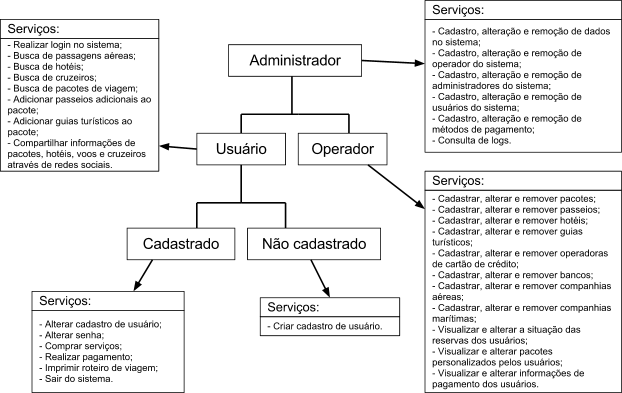
\includegraphics[scale=.55]{dia.png}
%               \caption{Diagrama HPV}
%\end{figure}

\section{Anexo}
\subsection{Tabelas VORD}


\subsection{Descrição dos serviços}

\begin{table}[htb]
\centering
\begin{tabular}{l|c|c|c|c|c|c}
\hline 
                & Fev & Mar & Abr & Mai & Jun & Jul \\ 
\hline \hline
Estudo          & X   & X  &      &     &     &     \\ 
\hline 
Implementação   & X   & X  &  X   &  X  &     &     \\ 
\hline 
Testes          &     &    &  X   &  X  &  X  &  X  \\ 
\hline 
Análise         &     &    &      &     &  X  &  X  \\ 
\hline 
Relatório       &     &    &      &     &  X  &  X  \\ 
\hline 
\end{tabular} 
\caption{Cronograma.\label{tab:cronograma}} 
\end{table}

% liste as referências bibliográficas citadas nas seções anteriores.
\addcontentsline{toc}{section}{\refname}
\bibliography{projeto}

\end{document}

